% tirlnx01 - Materiaal om het keuzevak Linux te geven 
% op de Hogeschool Rotterdam.
% Copyright (C) 2010 - 2011  Paul Sohier, Kevin van der Vlist
%
% This program is free software: you can redistribute it and/or modify
% it under the terms of the GNU General Public License as published by
% the Free Software Foundation, either version 3 of the License, or
% (at your option) any later version.
%
% This program is distributed in the hope that it will be useful,
% but WITHOUT ANY WARRANTY; without even the implied warranty of
% MERCHANTABILITY or FITNESS FOR A PARTICULAR PURPOSE.  See the
% GNU General Public License for more details.
%
% You should have received a copy of the GNU General Public License
% along with this program.  If not, see <http://www.gnu.org/licenses/>.
%
% Kevin van der Vlist - kevin@kevinvandervlist.nl
% Paul Sohier - paul@paulsohier.nl

\documentclass{beamer}

\mode<presentation>

\usepackage[dutch]{babel}
\usepackage{listings}
%\usepackage{beamerthemesplit}

\lstset{ %
  language=bash,                % choose the language of the code
  basicstyle=\footnotesize,       % the size of the fonts that are used for the code
  numbers=left,                   % where to put the line-numbers
  numberstyle=\footnotesize,      % the size of the fonts that are used for the line-numbers
  numbersep=5pt,                  % how far the line-numbers are from the code
  showspaces=false,               % show spaces adding particular underscores
  showstringspaces=false,         % underline spaces within strings
  showtabs=false,                 % show tabs within strings adding particular underscores
  frame=lr,	                % adds left and right lines
  tabsize=2,	                % sets default tabsize to 2 spaces
  captionpos=b,                   % sets the caption-position to bottom
  breaklines=true,                % sets automatic line breaking
  breakatwhitespace=false,        % sets if automatic breaks should only happen at whitespace
%  escapeinside={\%*}{*)},         % if you want to add a comment within your code
  morekeywords={esac,fi,elseif,*,...}            % if you want to add more keywords to the set
}
\usetheme{Berlin}
\useinnertheme{rounded}
\usecolortheme{rose}
\setbeamertemplate{navigation symbols}{} 

\title{Keuzevak Linux - Week 7}
\author{Paul Sohier \and Kevin van der Vlist}
\institute{Versie $1.0$}
\date{\today}

\begin{document}

\begin{frame}
  \titlepage
\end{frame} 

\begin{frame}
  \frametitle{Inhoud}
  \tableofcontents
\end{frame}

\section{Problemen oplossen}

\begin{frame}
  \frametitle{Problemen oplossen}
  \begin{itemize}
    \item<1-> Gestructureerd problemen oplossen
  \end{itemize}
\end{frame}

\begin{frame}
  \frametitle{Problemen oplossen - Analyse}
  \begin{itemize}
    \item<1-> Symptomen
    \item<2-> Raakvlaken: Binaries
    \item<3-> Reproduceerbaar?
  \end{itemize}
\end{frame}

\begin{frame}
  \frametitle{Problemen oplossen - Analyse - Reproduceerbaar}
  \begin{itemize}
    \item<1-> Minimale testcase
    \item<2-> Oplossing doorvoeren
    \item<3-> Oplossing documenteren
  \end{itemize}
\end{frame}

\begin{frame}
  \frametitle{Problemen oplossen - Analyse - Niet Reproduceerbaar}
  \begin{itemize}
    \item<1-> Overzicht invloeden onderlinge factoren
    \item<2-> Patroonherkenning
    \item<3-> Monitoren en snel ingrijpen
  \end{itemize}
\end{frame}

\section{Autotools}

\begin{frame}
  \frametitle{Autotools - Wat}
  \begin{itemize}
    \item<1-> Compileer omgeving
    \item<2-> Cross platform
    \item<3-> Dependency tracking
  \end{itemize}
\end{frame}

\begin{frame}
  \frametitle{Autotools - Waarom}
  \begin{itemize}
    \item<1-> Verschillende architectuur systemen 
    \item<2-> Verschillende inrichting systemen 
    \item<3-> Compiler opties
    \item<4-> Linker opties
    \item<5-> Scripting beperkingen / mogelijkheden
  \end{itemize}
\end{frame}

\begin{frame}
  \frametitle{Autotools - Hoe}
  \begin{itemize}
    \item<1-> In: generieke rules
    \item<2-> Uit: specifieke makefiles
  \end{itemize}
\end{frame}

\begin{frame}
  \frametitle{Autotools - Overview}
  \begin{figure}[H]
    \begin{center}
      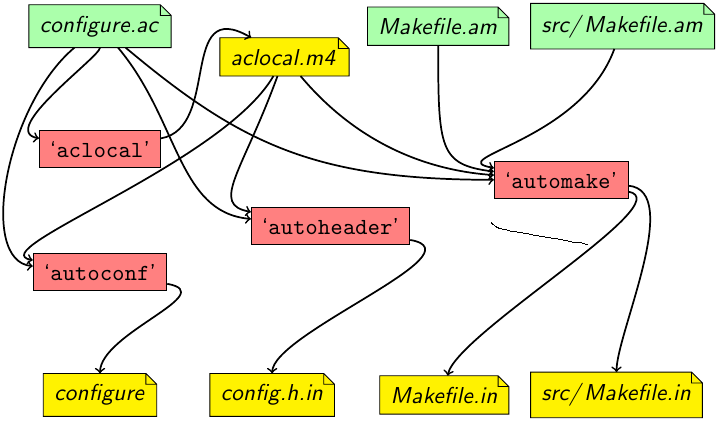
\includegraphics[scale=0.5]{images/auto_over}
    \end{center}
    \caption{Autotools Overview}
    \label{fig:auto_over}
  \end{figure}
\end{frame}

\section{Scripting demo}

\begin{frame}
  \frametitle{Scripting demo - Waarom}
  \begin{itemize}
    \item<1-> Waarom?
  \end{itemize}
\end{frame}

\begin{frame}
  \frametitle{Scripting demo - Demo}
  \begin{itemize}
    \item<1-> Emacs!
  \end{itemize}
\end{frame}

\begin{frame}[fragile]
  \frametitle{Scripting demo - Uitwerking - 1}
  \begin{lstlisting}
#!/bin/bash
if [ $# -ne 3 ]; then
    echo "Reverse polish calculator"
    echo "Gebruik: $0 2 3 x"
    exit 1
fi

  \end{lstlisting}
\end{frame}

\begin{frame}[fragile]
  \frametitle{Scripting demo - Uitwerking - 2}
  \begin{lstlisting}
case "$3" in 
    "x")
      antwoord=$(( $1 * $2 ));;
    "+")
      antwoord=$(( $1 + $2 ));;
    "-")
      antwoord=$(( $1 - $2 ));;
    "/")
      antwoord=$(( $1 / $2 ));;
    *)
      echo "Onbekende operator";;
esac
  \end{lstlisting}%$
\end{frame}

\begin{frame}[fragile]
  \frametitle{Scripting demo - Uitwerking - 3}
  \begin{lstlisting}
if [ -n "$antwoord" ]; then
    echo "Het antwoord van RPN: ($1 $2 $3) is: $antwoord"
fi;

exit 0
  \end{lstlisting}%$
\end{frame}

\end{document}
